\documentclass[main.tex]{subfiles} % Subfile-Class


% ============================================================================== %
%                            Subfile document                                    %
% ============================================================================== %

\begin{document}

% Template

\section{Liniensensor}
\label{anhang:Liniensensor}
Anbei folgen diverse Unterkapitel, welche Berechnungen sowie Messungen für die Erstellung eines Liniensensors beinhalten.

% ===================================================================================
\subsubsection*{Geometrische Überlegungen}
Abbildung~\ref{fig:Konzept_graphml} zeigt die konzeptionellen Überlegungen einer Messzelle des
Liniensensors. Gemäss dem Datenblatt hat der UV-Emitter (Sender) einen Abstrahlwinkel von 15° und der
Fototransistor (Empfänger) einen Einfallswinkel von 60°. Für eine möglichst störungsfreie Detektion muss auf dem Boden 
eine möglichst grosse Fläche des Empfänger-Kreises durch den Sender-Kreis ausgefüllt werden. Der passende
Abstand zwischen Liniensensor und Boden muss in der praxis mit Versuchsmessungen eruiert werden.\\
Diese einzelnen Messzellen sollen untereinander und von der Umwelt abgekapselt werden. Dies
mit der Begründung, dass die Fototransistoren, gegebenenfalls empfindlich auf
Umwelteinflüsse reagieren könnten. Daher wird ein Gehäuse für die Abschirmung von Umwelteinflüssen
konzipiert.

\begin{figure}[H]
    \centering
    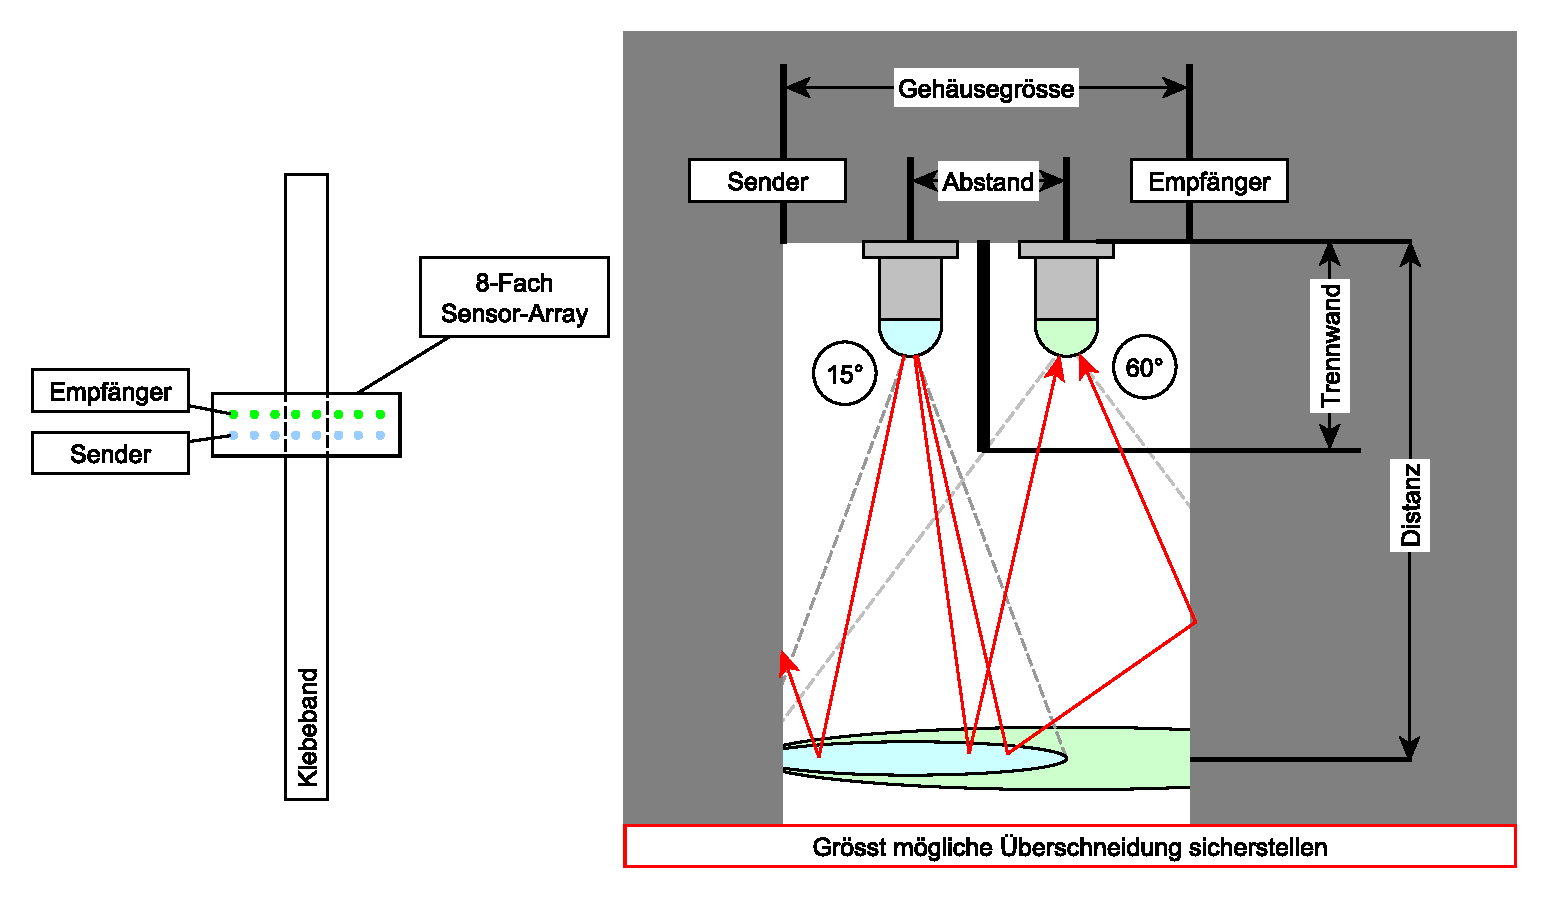
\includegraphics[width=0.75\textwidth]{./fig_Liniensensor/Konzept.pdf}
    \caption{Konzept des Liniensensors}~\label{fig:Konzept_graphml}
\end{figure}

% ===================================================================================

\subsubsection*{Dimensionierung Gehäuse}
Damit der Empfänger möglichst wenig auf Umwelteinflüsse reagiert, wird nun ein 
Gehäuse dimensioniert, welches den Sensor abschirmen soll. Die nachfolgende 
Abbildung~\ref{fig:Gehaeuse_Vermasst} zeigt eine Skizze, welche den Aufbau des Gehäuses repräsentiert.
In dieser Skizze wird jeder Emitter und Fototransistor von allen anderen abgeschottet. Die vier Löcher
passen genau auf das PCB des Liniensensors. Die Höhe des Gehäuses, stellt den Abstand zwischen Liniensensor
und dem Boden dar. Die grösste Stromdifferenz wurde in einer Höhe von 2.5 cm gemessen. Daher wird die Höhe
des Gehäuses auf 2.5 cm festgelegt.
Die isometrische Ansicht des Gehäuse ist in Abbildung~\ref{fig:Gehaeuse_Isometrisch} !!!!!Anpassen!!!!!!

\begin{figure}[H]
    \centering
    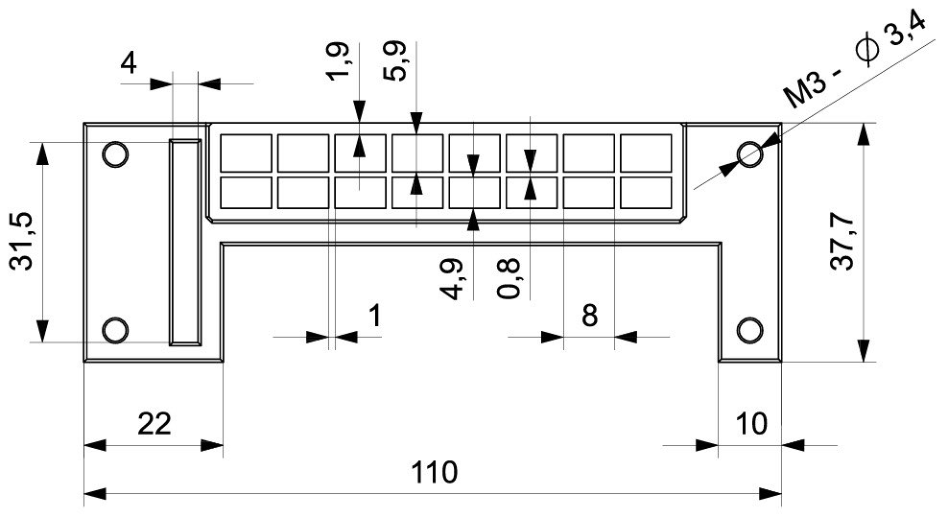
\includegraphics[width=0.75\textwidth]{./fig_Liniensensor/Gehaeuse_Vermasst.pdf}
    \caption{Vermassung des Gehäuses in Siemens NX}~\label{fig:Gehaeuse_Vermasst}
\end{figure}

\begin{figure}[H]
    \centering
    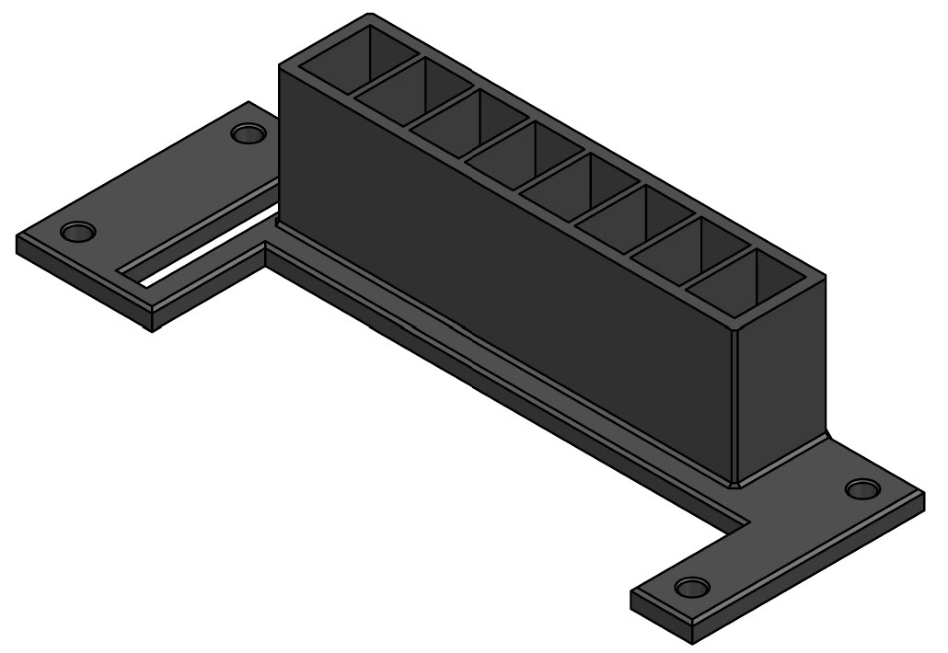
\includegraphics[width=0.75\textwidth]{./fig_Liniensensor/Gehaeuse_Isometrisch.pdf}
    \caption{Isometrische Ansicht des Gehäuses in Siemens NX}~\label{fig:Gehaeuse_Isometrisch}
\end{figure}

% ===================================================================================

\subsubsection*{Schema einer Messzelle}

\begin{figure}[H]
    \centering
    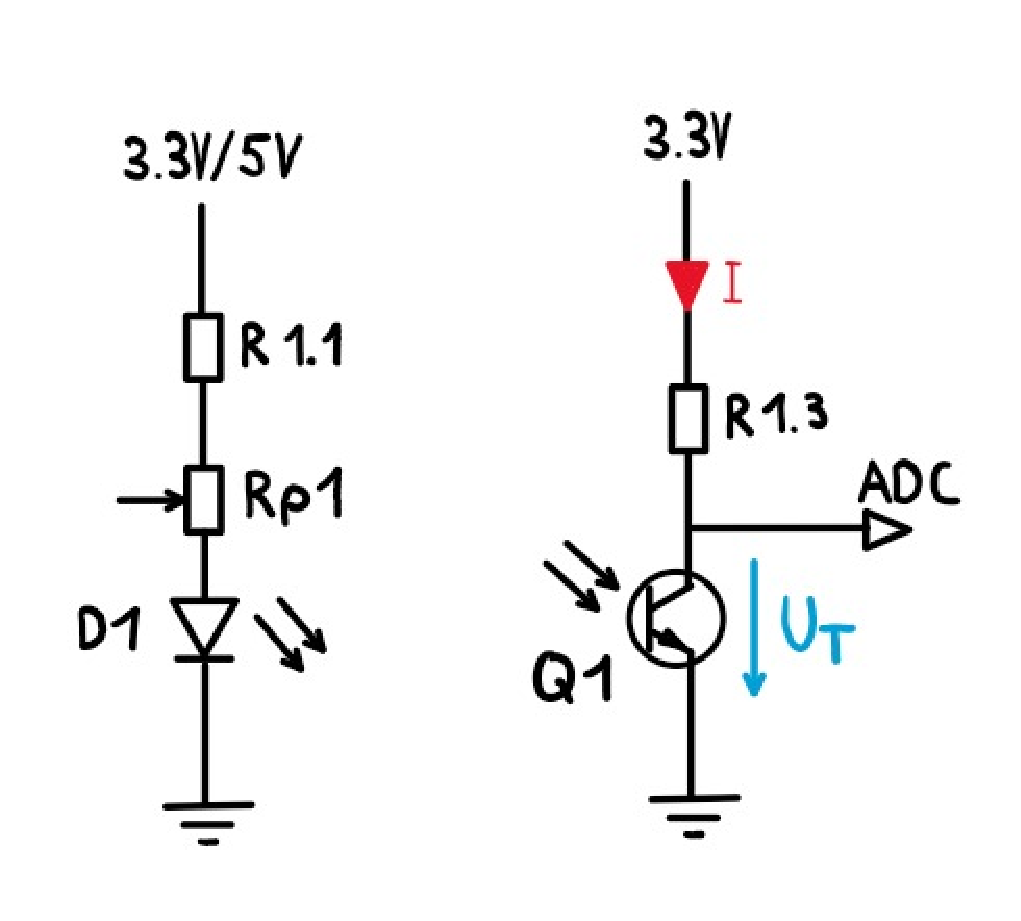
\includegraphics[width=0.5\textwidth]{./fig_Liniensensor/Schema_Messzelle_Liniensensor.pdf}
    \caption{Schema einer Messzelle}~\label{fig:Messzelle}
\end{figure}

Abbildung~\ref{fig:Messzelle} zeigt das Schema einer einzelnen Messzelle. Die Speisung hat eine Höhe von 5 V oder 3.3 V. 
Ausserdem ist als Sicherheitsmassnahme beim Messabgang über dem 
Fototransistor einen Platz für einen Widerstand eingebaut, damit bei allfälligen Stromspitzen der Strom 
limitiert werden könnte. Weil dies aber mit der verwendeten Auswertung nicht notwendig ist, wird ein
0 $\Omega$ Widerstand eingebaut. Die Potentiometer werden eingebaut, dass allfällige Bauteiltoleranzen
eliminiert werden können. In den folgenden Abschnitten wird dargestellt, wie die Werte der Komponenten $R_{1.1}$, $R_{p1}$ und $R_{1.3}$ 
dimensioniert werden.


% ======================================================================================
\subsubsection*{Wahl des Lichtspektrums}
Damit der Unterschied zwischen dem Wettkampfuntergrund und dem Klebeband möglichst 
drastisch hervorgehoben werden kann, ist zuerst eine Evaluierung des optimalen
Lichtspektrums nötig. Es werden nun Versuche dokumentiert, welche die Spannungen 
über dem Fototransistor im Infrarot-Spektrum (IR) und im Ultraviolett-Spektrum (UV) 
dokumentiert. Dabei wird für ersteres ein Emitter und ein Fototransistor im IR-Spektrum (beide 940 nm Peak-Wellenlänge)
verwendet. Beim Versuch im UV-Spektrum wird ein UV-Emitter (395nm Peak-Wellenglänge) mit einem Fototransistor (630nm Peak-Wellenlänge) 
im sichtbaren Spektrum verwendet. Dabei wird eine fluoreszierende Wirkung des Klebebandes 
vermutet.



%Im folgenden Abschnitt wird untersucht, ob sich das Infrarot-Spektrum oder das Ultraviolett-Spektrum besser für
%die Unterscheidung des Klebebands zum Wettkampfuntergrund eignet. Zuerst müssen aber alle Komponenten der Messzellen, 
%welche mit unterschiedlichen Wellenlängen emittierenden Dioden und Fototransistoren ausgestattet sind, berechnet werden.
%In Abbildung~\ref{fig:Schema_Messzelle_Liniensensor} ist die erste Messzelle von acht abgebildet. Für jede Messzelle
%gelten aber dieselben Werte.

%\begin{figure}[h!]
 %   \centering
  %  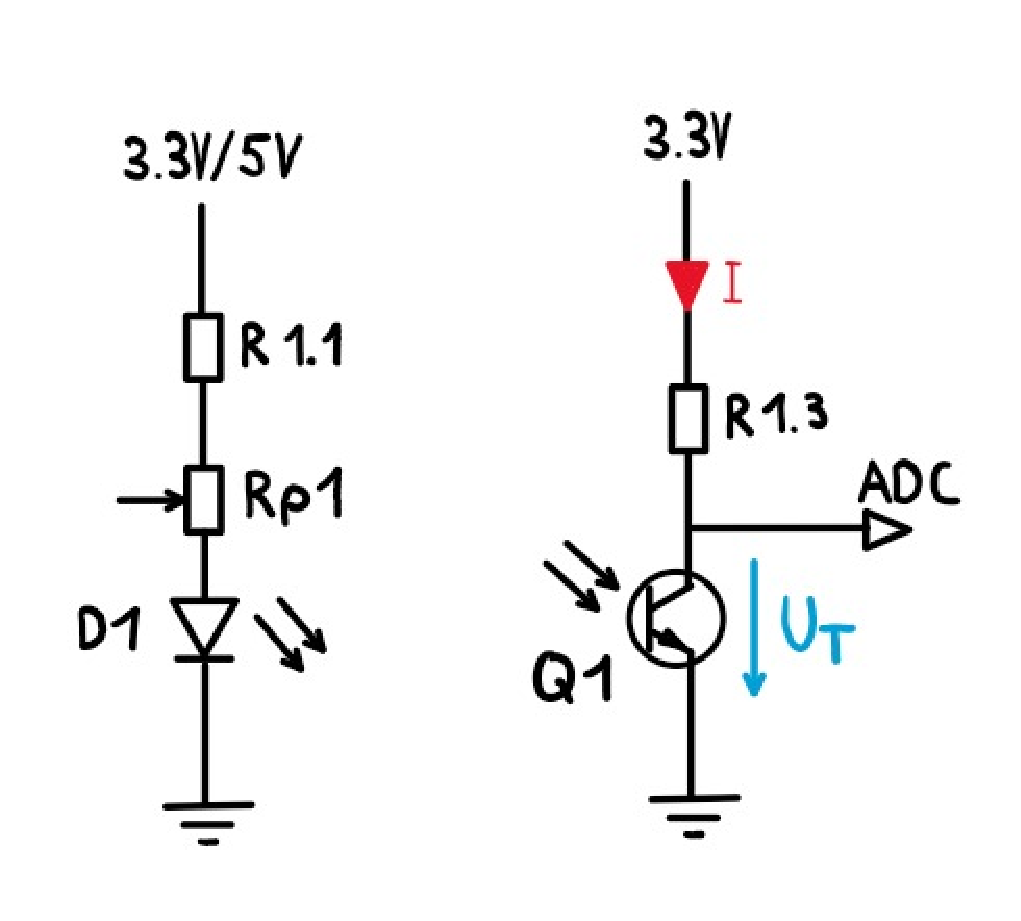
\includegraphics[width=0.5\textwidth]{./fig_Liniensensor/Schema_Messzelle_Liniensensor}
   % \caption{Erste Messzelle des Liniensensors, die restlichen sieben Messzellen sind identisch.}~\label{fig:Schema_Messzelle_Liniensensor}
%\end{figure}



\subsubsection*{Dimensionierung IR-Messzelle}
In diesem Abschnitt wird eine IR-Messzelle dimensionert. Gemäss Datenblatt kann über dem IR-Emitter von 1.3 V bis 2 V
abfallen. Die Speisespannung beträgt 3.3 V. Der maximale Strom beträgt 100 mA. Der Strom wird gewählt, dass er ungefähr im 
Bereich von 10 mA bis 60 mA fällt. Dies wurde so gewählt, das nicht zu viel Leistung verbraucht wird, aber der Emitter trotzdem 
mit genügen Strom versorgt wird. Daraus resultiert die folgende Widersandsberechnung:
\[
    R_{max} = \frac{U_q - U_{LED}}{I_{LEDmin}} = \frac{3.3 V - 1.3 V}{0.01A} = 200 \Omega
\]
\[
    R_{min} = \frac{U_q - U_{LED}}{I_{LEDmax}} = \frac{3.3 V - 1.3 V}{0.03A} = 33.33 \Omega
\]
Daraus resultiert ein Potentiometer $R_{p1}$ von 200 $\Omega$ und ein $R_{1.1}$ von 33 $\Omega$.
Der Widerstand $R_{1.3}$ kann erst später dimensioniert werden, weil der Strom durch ihn unklar ist.

%===========================================================================================================%

\subsubsection*{Dimensionierung UV-Messzelle}
In diesem Abschnitt wird die UV-Messzelle dimensioniert.
Über die Speisespannung von 5 V wird ein UV-Emitter mit Vorwiderstand bestromt. Der empfohlene Strom
wird Gemäss dem Datenblatt des UV-Emitters von 10 mA bis 20 mA vorgeschlagen. Ausserdem darf der Strom nicht 
30mA übersteigen. Daher resultiert: 

\[
    R_{max} = \frac{U_q - U_{LED}}{I_{LEDmin}} = \frac{5 V - 2.9 V}{0.01A} = 210 \Omega
\]
\[
    R_{min} = \frac{U_q - U_{LED}}{I_{LEDmax}} = \frac{5 V - 2.9 V}{0.03A} = 70 \Omega
\]
Daraus resultiert ein Potentiometer $R_{p1}$ von 200 $\Omega$ und ein $R_{1.1}$ von 82 $\Omega$, welches ungefähr im zuvor festgelegten
Strombereich liegt:
\[
    I_{max} = \frac{U_R}{R_{min}} = \frac{2.1}{82 \Omega} = 0.0256 A = 25.6 mA
\]
\[
    I_{min} = \frac{U_R}{R_{max}} = \frac{2.1}{282 \Omega} = 0.00745 A = 7.45 mA
\]
Aufgrund dieser Widerstandsaufteilung kann der Strom ungefähr in dem empfohlenen Bereich frei eingestellt werden.
Der Widerstand $R_{1.3}$ kann erst später dimensioniert werden, weil der Strom durch ihn unklar ist.

\subsubsection*{Versuchsmessungen}
Bei den beiden oben dimensionierten Varianten wird je eine Messzelle auf ein PCB gelötet und dann der Strom durch den
Fototransistor gemessen. Die gemessenen Werte sind in der folgenden Tabelle~\ref{tab:Strommessungen_einzeln} festgehalten. Dabei resultierte der 
Abstand von ungefähr 2.7mm von Messfläche zum Liniensensor. Das Potentiometer wird in die Mitte eingestellt, sprich
auf 100 $\Omega$.

\begin{table}[h]                                    
    \centering
    \begin{tabular}{|c|c|c|c|c|c|c|}                        
        \hline
        \textbf{Lichtspektrum} & \textbf{Strom Klebeband [mA]}        & \textbf{Strom Fuge [mA]}    & \textbf{Strom Fliese [mA]}\\ \hline
        Infrarot              & 1.368                                 & 1.248                        & 1.92                       \\ \hline
        Ultraviolett          & 0.2024                                & 0.0691                       & 0.0494                     \\ \hline

        \end{tabular}
\caption{Strom durch die beiden Fototransistor in verschiedenen Lichtspektren}
\label{tab:Strommessungen_einzeln}
\end{table}


Aus der Tabelle ist zu sehen, dass im UV-Spektrum der Strom über dem Klebeband geringerer ist als beim IR-Spektrum. Jedoch ist der Differenzfaktor beim UV-Spektrum zu den 
verschiedenen Messuntergründen etwa doppelt so hoch im Vergleich zum IR-Spektrum. Aufgrund dieser Messresultate wird auf das UV-Spektrum zurückgegriffen.


\subsection*{Dimensionierung des Widerstandes $R_{1.3}$}
In dem oberen Abschnitt wurde der Strom durch einen Fototransistor gemessen. Wie schon oben erwähnt, wird aufgrund der besseren Messwerte auf das UV-Spektrum
zurückgegriffen. Jedoch wurde für den Versuch nur eine Messzelle gemessen. Mit nun acht Messzellen beeinflussen sich die Messzellen trotz möglichst präziser 
Abschirmung immer noch gegenseitig. Das heisst, mehr Licht entspricht einer höheren ansteuerung der Basis des Fototransistors und somit einen höheren Strom. 
Deswegen muss dieser nun neu gemessen werden. Bei allen acht Messzellen werden die verschiedenen Ströme auf allen Messuntergründen gemessen. In der Tabelle~\ref{tab:Strommessungen_alle} sind die maximal
gemessenen Ströme auf der Fliese und der Fuge ersichtlich. Mit den Potentiometern werden die Ströme durch die Emitter so eingestellt, dass sie auf dem Klebeband durch den Fototransistor immer 
etwa gleich hoch ausfallen (480 mA). Dies mit der Begründung, dass ein möglichst einheitlicher Strom durch den Fototransistor fliesst, wenn er sich auf dem Klebeband befindet.

\begin{table}[h]                                    
    \centering
    \begin{tabular}{|c|c|c|c|c|c|c|}                        
        \hline
        \textbf{Messuntergrund} & \textbf{Strom in [mA]}        \\ \hline
        Klebeband               & 0.48                          \\ \hline
        Fliese                  & 0.34                          \\ \hline
        Fuge                    & 0.23                          \\ \hline

        \end{tabular}
\caption{Strom durch den Fototransistor auf den verschiedenen Messuntergründen}
\label{tab:Strommessungen_alle}
\end{table}

Weil nun die Ströme durch den Fototransistor bekannt sind, kann nun der passende Widerstandswert für $R_{1.3}$ berechnet werden. Weil der Strom
durch den Fototransistor auf dem Klebeband nie ganz genau identisch sein wird, wird ein Schwellwert angenommen. Es wird nun ein Strom $I_{\text{F}}$ von $400 \, \mu A$
angenommen. Dieser Wert bietet noch genügend Differenz zum Fliesen-/Fugenstrom. Daher kann der Widerstand $R_{1.3}$ berechnet werden.

\[
    R_{1.3} = \frac{U_q}{I_{\text{Ph}}} = \frac{3.3 \, \text{V}}{400 \, \mu \text{A}} = 8.25 \, \text{k}\Omega
\]


Daraus resultiert ein Widerstand $R_{1.3}$ von 8200 Ohm. Das bedeutet, sobald der Strom grösser als $400 \, \mu A$ ist, geht die Spannung über dem
Fototransistor annähernd zu Ground. Unter dem Schwellwert wird ein Spannungsoffset registriert.

\subsection*{Messwerte des Liniensensors}
Um diese Berechnungen zu verifizieren, wird der Liniensensor mit
einem Arduino geprüft. Die Auswertung des Arduinos ist in der Tabelle~\ref{tab:Spannungsauswertung_Arduino} dargestellt.
\begin{table}[h]                                    
    \centering
    \begin{tabular}{|c|c|c|c|c|c|c|}                        
        \hline
        \textbf{Kennzahl aus Software} & \textbf{Spannung in [V]}        \\ \hline
        0                      & 0V                                     \\ \hline
        205                    & 1V                                     \\ \hline
        1023                   & 5V                                     \\ \hline

        \end{tabular}
\caption{Spannungsauswertung des Arduinos über dem Fototransistor}
\label{tab:Spannungsauswertung_Arduino}
\end{table}\\

Es kann also ein Spannungsbereich von 0 V bis 5 V über dem Fototransistor ausgewertet werden. Anbei sind nun einige Versuchsmessungen dokumentiert.\\\\


Bei der Abbildung~\ref{fig:Auswertung_Klebeband_zu_Fuge} ist der Vergleich Fliese (oben) zu Klebeband (unten) ersichtlich. Die Werte auf dem Boden schwanken zwar, 
sind aber nie unter 350, also sprich 1.707 V. Die Werte auf dem Klebeband werden jedoch immer sauber gegen Ground gezogen.

\begin{figure}[h!]
    \centering
    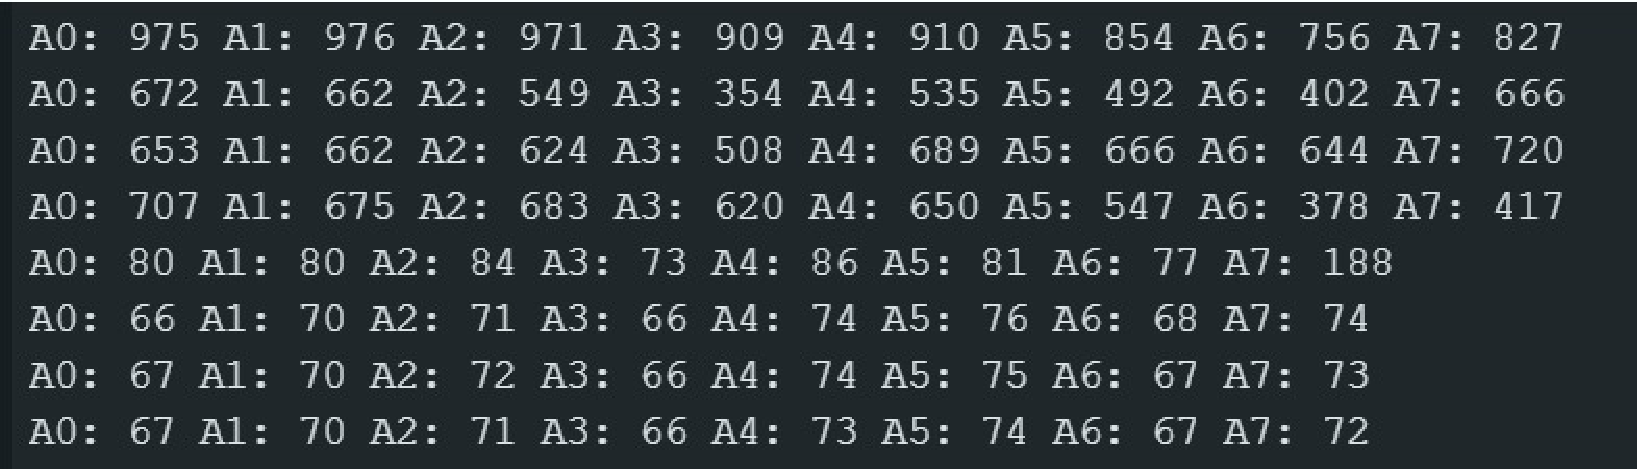
\includegraphics[width=0.75\textwidth]{./fig_Liniensensor/Auswertung_Klebeband_zu_Fuge}
    \caption{Vergleich der Kennzahlen von Fliese (oben) und Klebeband (unten) des Arduinos}~\label{fig:Auswertung_Klebeband_zu_Fuge}
\end{figure}

Die Abbildung~\ref{fig:Auswertung_Strecke} zeigt, wie eine mögliche Strecke getrackt werden kann. Dabei wird vorallem A3 gegen Ground gezogen.
Ausserdem kann man sehen, dass A2 und A4 auch das Klebeband tracken. Jedoch nicht so deutlich. Dies liegt daran, dass diese beiden Messzellen nicht
direkt auf das Klebeband ausgerichtet sind.

\begin{figure}[h!]
    \centering
    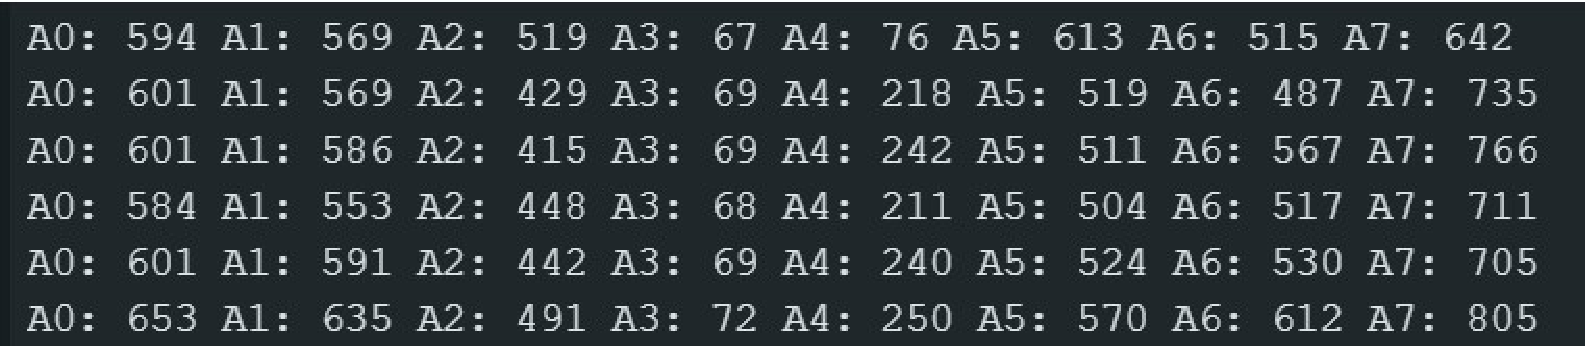
\includegraphics[width=0.75\textwidth]{./fig_Liniensensor/Auswertung_Strecke}
    \caption{Vergleich der Kennzahl Klebeband (vorallem A3) und der Fliese}~\label{fig:Auswertung_Strecke}
\end{figure}

In Abbildung~\ref{fig:Auswertung_mit_Fuge} wird die Auswertung aufgezeigt, bei der die Fuge auch miteinbezogen wurde. Diese ist bei dem Pin A2 leicht
sichtbar. Fällt aber fast nicht auf. Im Vergleich zu A6, bei dem das Klebeband angezeigt wird. Die restlichen Pins stellen die Fliese dar.

\begin{figure}[h!]
    \centering
    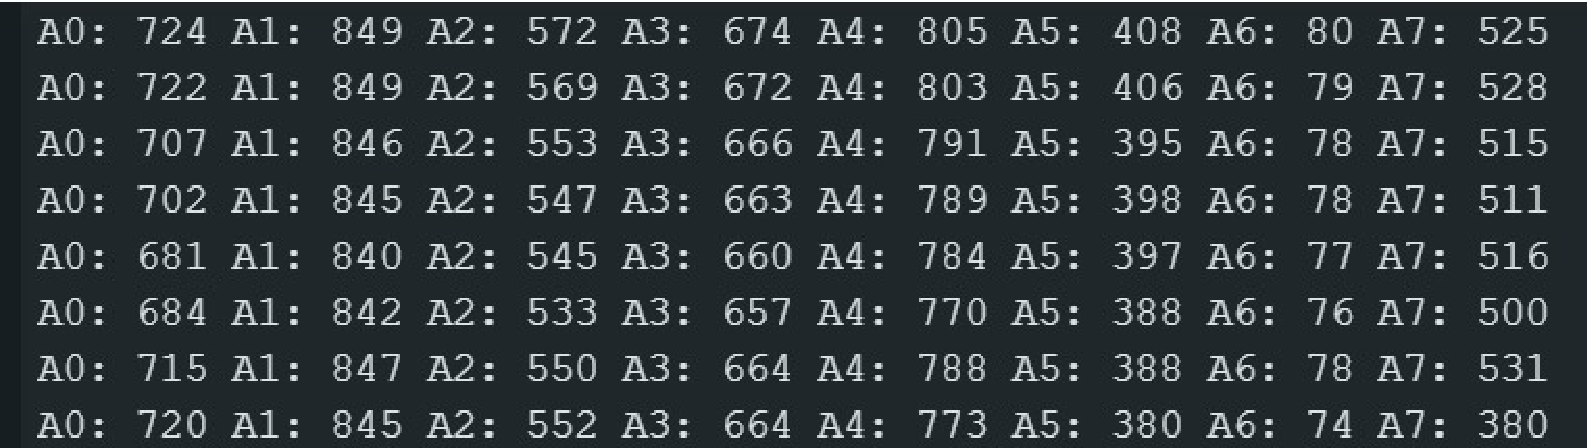
\includegraphics[width=0.75\textwidth]{./fig_Liniensensor/Auswertung_mit_Fuge}
    \caption{Vergleich der Kennzahl Fuge (A6) und dem Klebeband (A6) umrandet von der Fliese}~\label{fig:Auswertung_mit_Fuge}
\end{figure}

%===========================================================================================================%
\end{document}
